\documentclass[8pt,CJK]{beamer}

%% Setup appearance:
%\usetheme{Antibes}
%\usetheme{Warsaw}
\usetheme{CambridgeUS}

\usecolortheme{dove}
%\setbeamerfont*{frametitle}{size=\normalsize,series=\bfseries}
%\setbeamertemplate{navigation symbols}{}

\usepackage[english]{babel}
\usepackage[latin1]{inputenc}
\usepackage[T1]{fontenc}
\usepackage{CJK}
\usepackage{tikz,layout}
\usepackage{mathptm}


% Author, Title, etc.

\title[]
{
 ���ิ�������ͬ��
}

\author[Wang~Jingyi]
{
  ������\inst{1}
}

\institute[Shenzhen University]
{
  \inst{1}
  ��ѧ ������ѧѧԺ,���ڴ�ѧ
}

\date[2012]{��ҵ���Ĵ��, 2012-5-10}



% The main document

\begin{document}
\begin{CJK*}{GBK}{song}
\begin{frame}
  \titlepage
\end{frame}

\begin{frame}{Outline}
  \tableofcontents
\end{frame}


\section{����}

\subsection{The Complex Network  and the Synchronization}
\begin{frame}
  \layout
\end{frame}
    \begin{frame}
        \frametitle{What is Complex Network?}

            In the context of network theory, a complex network is a network (graph) with non-trivial topological features��features that do not occur in simple networks such as lattices or random graphs but often occur in complete graphs. The study of complex networks is a young and active area of scientific research inspired largely by the empirical study of real-world networks such as computer networks and social networks.\\

            Two well-known and much studied classes of complex networks are scale-free networks and small-world networks, whose discovery and definition are case-studies in the field.
    \end{frame}

    \begin{frame}
        \frametitle{scale-free networks}
        \begin{itemize}
          \item Scale-free networks show a power law degree distribution like many real networks.
          \item rich get richer
          \item The mechanism of preferential attachment has been proposed as a mechanism to explain power law degree distributions in some networks.
        \end{itemize}
    \end{frame}
    \begin{frame}
        \begin{figure}
          % Requires \usepackage{graphicx}
          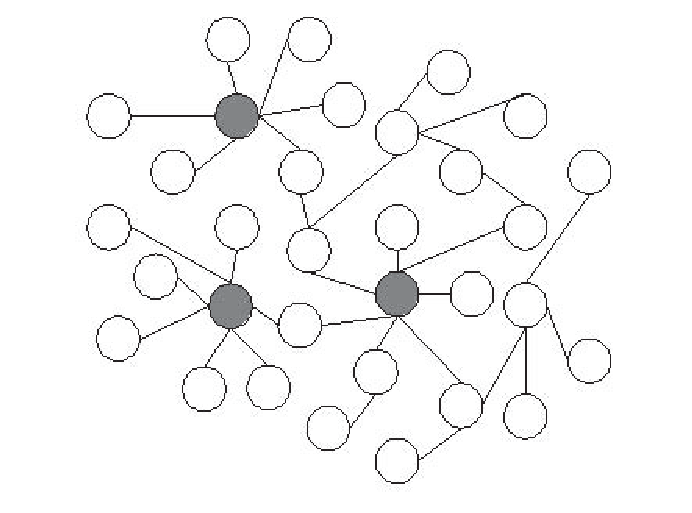
\includegraphics[width=2.5in]{Figure/fig1.eps}\\
          \caption{A scale-free network}\label{}
        \end{figure}
\begin{align}\label{sys:pin}
        dx_i(t)=&\Bigl\{f(t,x_i(t),x_i(t-\tau(t)))+\sum_{j=1,i \neq j}^N a_{ij}(r_{a_{ij}}(t))\Sigma (x_j(t)-x_i(t))\notag\\
                &+ \sum_{j=1,i \neq j}^N b_{ij}(r_{b_{ij}}(t))\Sigma (x_j(t-\tau_c(t))-x_i(t-\tau_c(t)))+u_i(t)\Bigr\}dt\notag\\
                &+\sigma_i(t,x(t),x(t-\tau(t)),x(t-\tau_c(t)),r_{\sigma_i}(t))dw_i(t),\quad i=1,2,\ldots,N,
    \end{align}
    \end{frame}

    \begin{frame}
        \frametitle{small-world networks}
        Small-world networks tend to contain neighborhood, and near-neighborhood, meaning sub-networks which have connections between almost any two nodes within them. This follows from the defining property of a high cluster coefficient.  Most pairs of nodes will be connected by at least one short path.
        \end{frame}
        \begin{frame}
        \begin{figure}
          % Requires \usepackage{graphicx}
          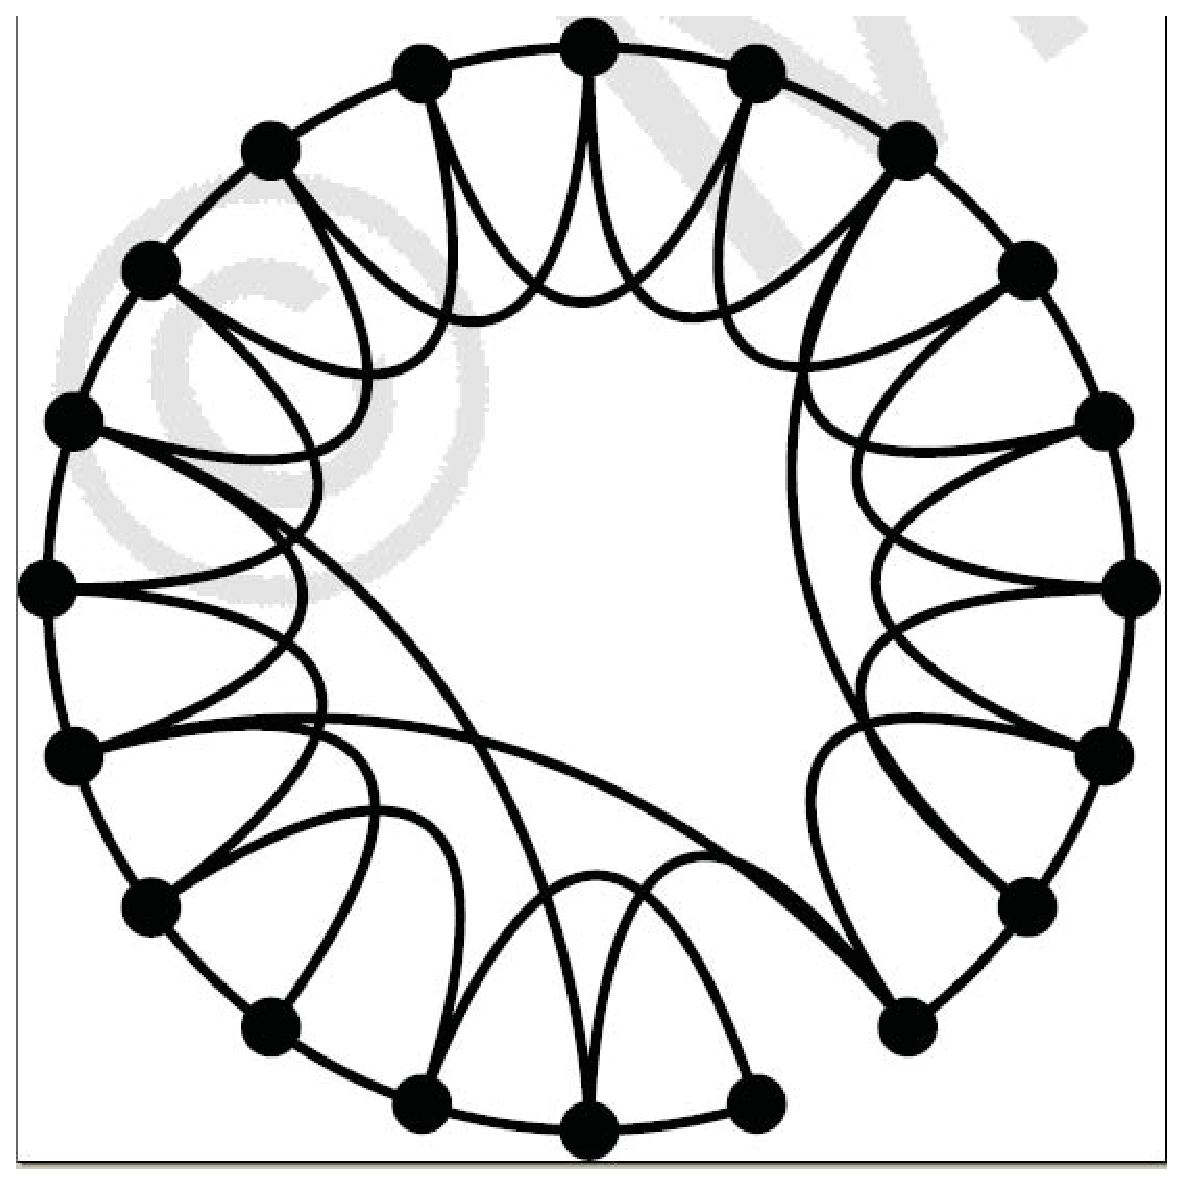
\includegraphics[width=2.5in]{Figure/fig2.eps}\\
          \caption{A small-world network}\label{}
        \end{figure}
    \end{frame}
    \begin{frame}
      Both are characterized by specific structural features��power-law degree distributions for the former and short path lengths and high clustering for the latter. However, as the study of complex networks has continued to grow in importance and popularity, many other aspects of network structure have attracted attention as well.
    \end{frame}
    \begin{frame}
        \frametitle{What is Synchronization?}
        The origin of the word synchronization is a Greek root ($\sigma\upsilon\gamma$ $\chi\rho o \nu o\varsigma$ which means ��to share the common time��). The original meaning of synchronization has been maintained up to now in the colloquial use of this word, as agreement or correlation in time of different processes.
        \begin{definition}
            In mathematics, \alert{synchronization} can be defined as a process wherein two (or many) dynamical systems adjust a given property of their motion to a common behavior as time goes to infinity, due to coupling or forcing.
        \end{definition}
    \end{frame}

    \begin{frame}
        \frametitle{Synchronization Patterns}
       Many different synchronization states have been studied in the past 10 years, for example complete synchronization, phase synchronization, lag  synchronization, generalized synchronization, imperfect phase synchronization, and almost synchronization and cluster synchronization.
    \end{frame}




\subsection{Cluster Synchronization}
    \begin{frame}{What is Cluster Synchronization?}
        \begin{definition}
          \alert{cluster synchronization} is observed when the dynamical nodes synchronize each other in each group (formed by certain partition rules), but no synchronization appears between any two different groups.
        \end{definition}

        Cluster Synchronization was the first discovered and is the simplest form of synchronization in chaotic systems. It consists in a perfect hooking of the chaotic trajectories of two systems which is achieved by means of a coupling signal, in such a way that they remain in step with each other in the course of the time.
    \end{frame}




\section{How to achieve synchronization and cluster synchronization}


    \begin{frame}
    \frametitle{If you are interesting, Reading...}

        {\tiny [1] S. Boccaletti, J. Kurths, G. Osipov, D. L. Valladares, and C. S. Zhou, The synchronization of chaotic systems, Phys. Rep., vol. 366, no. 1/2,pp. 1-101, Aug. 2002.}

        {\tiny [2] Vladimir N. Belykh, Igor V. Belykh, and Erik Mosekilde, Cluster synchronization modes in an ensemble of coupled chaotic oscillators, Phys. Rev. E 63, 036216 (2001)}

        {\tiny [3] Kaihua Wang Xinchu Fu and Kezan Li, Cluster synchronization in community networks with nonidentical nodes,CHAOS 19, 023106 (2009)}

        {\tiny [4] T. P. Chen, X. W. Liu, and W. L. Lu, Pinning Complex Networks by a Single Controller, IEEE Transactions on Circuits and Systems-I: Regular Papers, vol.54, no.6, pp.1317-1326, 2007}

        {\tiny [5] Zhongjun Ma, Zengrong Liu, and Gang Zhang, A new method to realize cluster synchronization in connected chaotic networks, Chaos 16, 023103 (2006)}

        {\tiny [6] Wei Wu, Wenjuan Zhou, and Tianping Chen, Cluster Synchronization of Linearly Coupled Complex Networks Under Pinning Control, IEEE Transactions on Circuits and Systems-I: Regular Papers, vol. 56, no. 4,pp829-839. APRIL 2009}
    \end{frame}
    \begin{frame}
         \frametitle{Reading...}
        {\tiny [7] Wenlian Lu,Bo Liu, Tianping Chen, Cluster synchronization in networks of coupled noidentical dynamical system, Chaos 20, 013120 (2010)}

        {\tiny [8] W. L. Lu, B. Liu and T. Chen, Cluster synchronization in networks of distinct groups of maps,Eur. Phys. J. B, vol.77, no.2, pp.257-264, DOI: 10.1140/epjb/e2010-00202-7(2010)}


        {\tiny [9] W. L. Guo, F. Austin, S. H. Chen, Global synchronization of nonlinearly coupled complex networks with non-delayed and delayed coupling, Commun Nonlinear Sci Numer Simulat, vol.15, pp.1631-1639, 2010}

        {\tiny [10] W.Wu and T. P. Chen, Global synchronization criteria of linearly coupled neural network  systems with time-varying coupling, IEEE Trans. Neural Netw., vol. 19, no. 2, pp. 319-332, Feb. 2008.}

        {\tiny [11]  Zhao J C, Lu J A, Wu X Q. Pinning control of general complex dynamical networks with optimization. Sci China Inf Sci, 2010, 53: 813-822, doi: 10.1007/s11432-010-0039-3}
    \end{frame}




\section{Some Numerical Simulation}
\subsection{No Synchronization}
    \begin{frame}
         \frametitle{Nodes states without Coupling}
         \begin{figure}
            % Requires \usepackage{graphicx}
            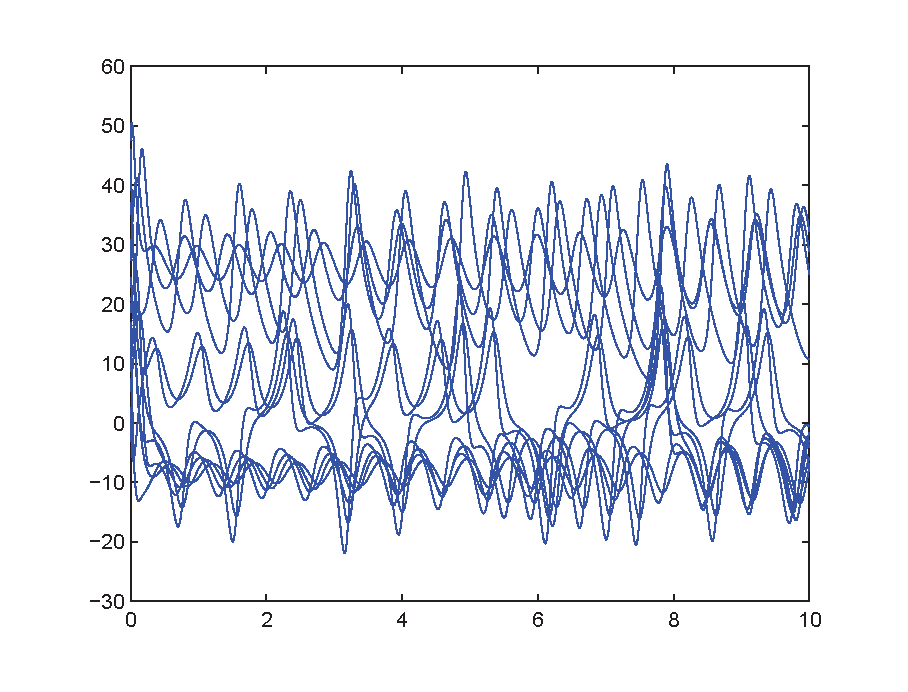
\includegraphics[width=2.5in]{Figure/uncoupling.eps}\\
            \caption{Nodes states without Coupling}
         \end{figure}
    \end{frame}
\subsection{Synchronization}
    \begin{frame}
         \frametitle{Nodes states of Synchronization}
         \begin{figure}
            % Requires \usepackage{graphicx}
            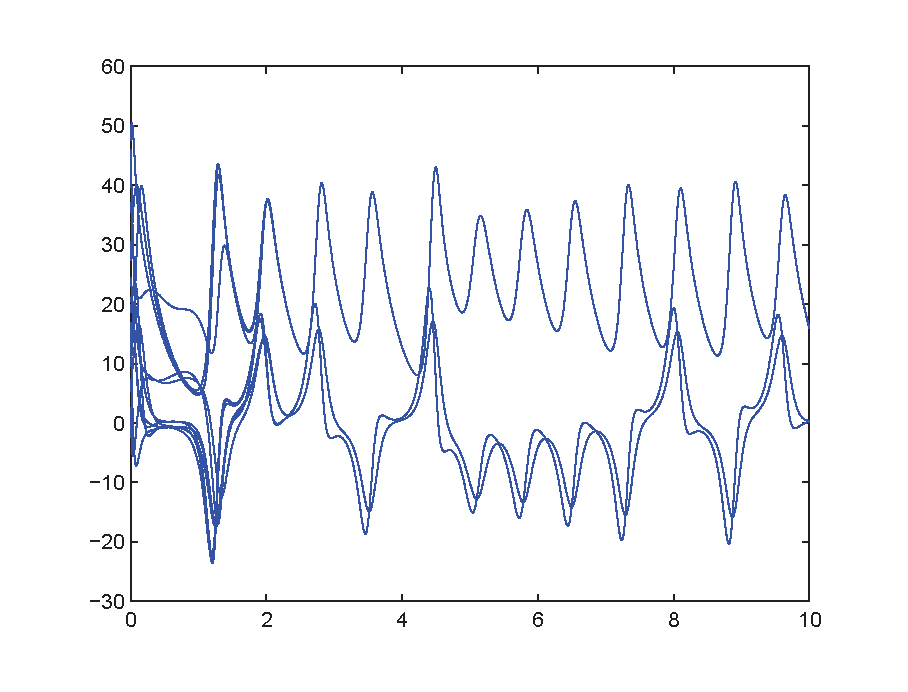
\includegraphics[width=2.5in]{Figure/coupling.eps}\\
            \caption{Nodes states of Synchronization}
         \end{figure}
    \end{frame}
\subsection{Cluster Synchronization}

    \begin{frame}
         \frametitle{Nodes states of Cluster Synchronization}
         \begin{figure}
            % Requires \usepackage{graphicx}
            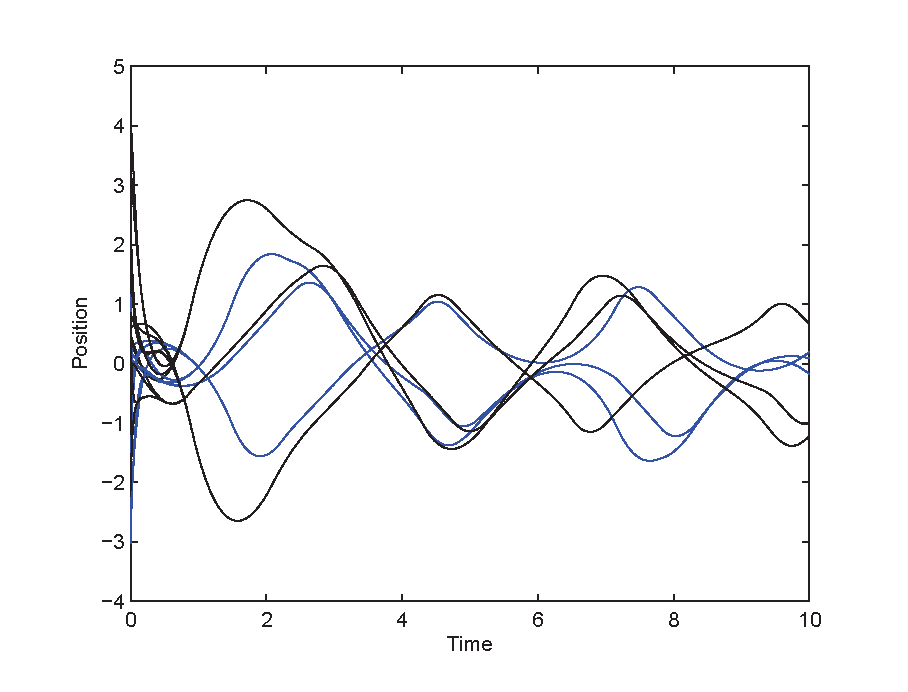
\includegraphics[width=2.5in]{Figure/clustersynchronization.eps}\\
            \caption{Nodes states of  Cluster Synchronization}
         \end{figure}
    \end{frame}

\end{CJK*}
\end{document}


